\section{Zielsetzung}
Mit der Hilfe von Brückenschaltungen lässt sich jede physikalische Größe, die sich
eindeutig als Widerstand darstellen lässt messen.
Dies wird mit verschiedenen Arten von Brückenschaltungen durchgeführt.

\secion{Theorie}
Allgemein wird bei Brückenschaltungen die Potentialdifferenz zwischen zwei
Punkten zweier getrennter stromduchflossener Leiter in Abhängigkeit des
Widerstandsverhältnisses. Daher hat sie im allgemeinen eine Schaltung wie in
Abbildung \ref{fig:allg} dargestellt.
\begin{figure}[H]
  \centering
  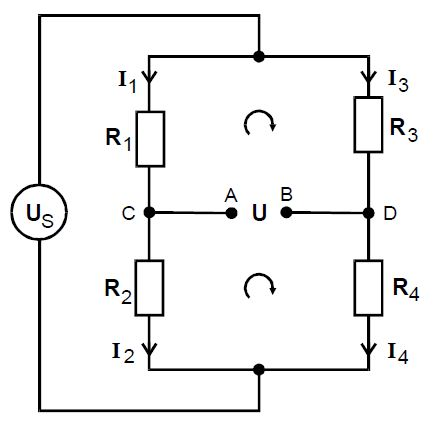
\includegraphics{allg.JPG}
  \caption{Allgemeine Schaltung einer Brückenschaltung.}
  \label{fig:allg}
  \cite{skript}
\end{figure}
Als Brückenspannung wird die zwischen den Punkten A und B auftretende Spannung
bezeichnet. Sie lässt sich mit Hilfe der Kirchhoffschen Gestze berechnen.
Dabei lautet das 1. Kirchhoffsche Gesetz: In einem Knotenpunkt muss die
Summe aus allen Strömen (zufließend und abfließend) Null ergeben.
\begin{equation}
  \sum_{i} I_{i} = 0
  \ref{eqn:kirch1}
\end{equation}
Das zweite Kirchhoffsche Gesetz lautet: In jeder Masche eines Stromkreises
ist die Summer über die Spannungen gleich Null.
\begin{equation}
  \sum_{i} U_{i} =0
  \ref{eqn:kirch2}
\end{equation}

Aus diesen Gesetzen lässt sich folgender Zusammenhang für die Brückenspannung
herleiten:
\begin{equation}
  U=\frac{R_{2}R{3}-R_{1}R{4}}{(R_{3}+R_{4})(R_{1}+R_{2})}U_{s}.
  \ref{eqn:ubrücke}
\end{equation}
Hier lässt sich erkennen, dass die Brückenspannung für die Bedingung
\begin{equation}
  R_{2}R_{3}=R_{1}R_{4}
  \ref{eqn:rbrücke}
\end{equation}
verschwindet. Ist das der Fall, wird die Brücke als abgeglichene Brücke bezeichnet.
Da die Abgleichbedingung nur von den Widerständen abhängig ist, kann durch
variieren dreier bekannter Widerstände (z.B. R_{2},R_{3},R_{4})ein unbekannter
Widerstand (z.B. R_{1}) ausgemessen werden. Die Genauigkeit der Messung ist davon
abhängig wie genau die Widerstände (z.B. R_{2},R_{3},R_{4}) bekannt sind und wie
ganau der Wert "Null" als Brückenspannung eingestellt werden kann.
Die Abgleichbedingung ist unabhängig von der Speisespannung U_{s}, da
die Brückenspannung aber proportional zu dieser ist, sollte sie
dennnoch hoch gewählt werden, um eine hohe Abgleichempfindlichkeit zu erhalten.

\noindent Betrachtet man eine Brückenschaltung, die auch Kapatitäten und
Induktivitäten enthält, verwendet man bei der Berechnung komplexe
Widerstände, auch Impedanzen genannt. Diese haben die allgemeine Form
\begin{equation}
  Z = X + iY
\end{equation}
wobei $X$ der Wirkwiderstand und $Y$ der Blindwiderstand ist. Für einen
Kondensator $C$, eine Induktivität $L$, und eine ohmschen Widerstand $R$
ergeben sich folgende Impedanzen.
\begin{align*}
  Z_{C} &= \frac{-i}{\omega C}
  Z_{L} &= i \omega L
  Z_{R} &= R
\end{align*}

Für eien Brückenschaltund mit Impedanzen lautet die Abgleichbedingung äqivalent zu
\ref{eqn:rbrücke}:
\begin{equation}
  Z_{2}Z_{3}=Z_{1}Z_{4}.
  \ref{eqn:zbrücke}
\end{equation}
Imaginäre Zahlen sind im Allgemeinen genau dann gleich, wenn der Real- und
Imaginärteil gleich sind. Daher muss für eine abgeglichene Wechselspannungsbrücke
die Brückenspannung nach Betrag und Phase verschwinden.
Deshalb besitzt jede Wechselstrombrücke zwei voneinander unabhängige Stellglieder.

\subsection{Wheatstonsche Brücke/Widerstandsmessbrücke}
\noindent Diese Brückenschaltung kann mit Gleich- und Wechselstrom betrieben werden,
da sie nur ohmsche Widerstände enthält.
\begin{figure}[H]
  \centering
  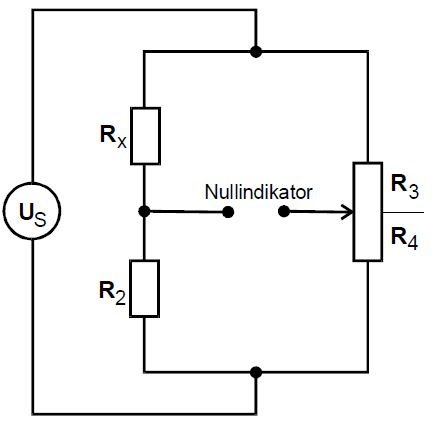
\includegraphics{widerstand.JPG}
  \caption{Wheatstonsche Brückenschaltung.}
  \label{fig:widerstand}
  \cite{skript}
\end{figure}

\noindent Mit dieser Schaltung kann der unbekannte Widerstand $R_{x}$ gemessen werden.
Nach Gleichung \red{eqn:rbrücke} gilt die Bedingung
\begin{equation}
  R_{x}= R_{2}\frac{R_{3}}{R_{4}}.
  \label{eqn:rx}
\end{equation}
%$R_{x}$ ist von dem Verhältnis von R_{3} zu R_{4} abhängig, diesen wird auch
%als Poentiometer bezeichnet.
\subsection{Kapatitätsmessbrücke}
Da es in einem realen Kondensator durch die Umwandlung von elektrischer Energie in
Wärme zu dielektrischen Verlusten kommt, wird ein Ersatzschaltbild eingeführt.
In diesem Erstzschaltbild wird der Kondensator mit einem (fiktiven) ohmschen Widerstand
in Reihe geschaltet. Somit ergibt sich für einen realen Kondensator:
\begin{equation*}
  Z_{C_{\text real}}=R-\fac{i}{\omega C}.
  \label{eqn:zcreal}
\end{equation*}
\begin{figure}[H]
  \includegraphics{kapatitat.JPG}
  \caption{Kapazitätsmessbrücke für Kondensatoren mit dielektrischen Verlusten}
  \label{fig:kapazitat}
  \cite{skript}
\end{figure}
Mit dieser Brücke kann eine unbekannte Kapazität $C_{x}$ gemessen werden.
Dabei ist neben dem Potentiometer ($\frac{R_{3}}{R_{4}}$) auch der Widerstand
$R_{2}$ veränderlich.
Aus der Abgleichbedingung \ref{eqn:zbrücke} ergibt sich
\begin{align}
  R_{x} &=R_{2}\frac{R_{3}}{R_{4}} \text und
  C_{x} &=C_{2}\frac{R_{4}}{R_{3}}.
\end{align}

\subsection{Induktivitätsmessbrücke}
 Auch eine reale Induktivität wandelt einen Tei der Enrgie in Wärme um, daher wird äquivalent
 zum Kondensator ein Erstzschaltbild eingeführt, in dem ein ohmscherwiderstand in Reihe
 zur Induktivität geschaltet wird.
 Daraus ergibt sich für die Impedanz einer realen Spule:
 \begin{equation}
   Z_{L_{\text real}}= R + i\omega L.
   \label{zlreal}
 \end{equation}

\begin{figure}[H]
  \centeribg
  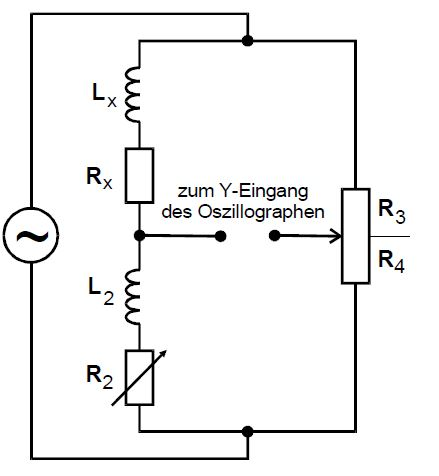
\includegraphics{induktivitat.JPG}
  \caption{Messbrücke für reale Induktivitäten.}
  \label{fig:induktivitat}
\end{figure}
Aus der Abgleichbedingung \ref{eqn:zbrücke} ergibt sich
\begin{align}
  R_{x} &=R_{2}\frac{R_{3}}{R_{4}} \text und
  L_{x} &=L_{2}\frac{R_{3}}{R_{4}}.
\end{align}







\label{sec:Theorie}

%\cite{sample}
